\documentclass[journal]{IEEEtran}

% Packages
\usepackage{cite}
\usepackage{amsmath,amssymb,amsfonts}
\usepackage{graphicx}
\usepackage{textcomp}
\usepackage{xcolor}
\usepackage{booktabs}
\usepackage{multirow}
\usepackage{hyperref}
\usepackage{listings}
\usepackage{algorithm}
\usepackage{algorithmic}
\usepackage{float}

% Listings style
\lstset{
  basicstyle=\footnotesize\ttfamily,
  breaklines=true,
  frame=single,
  numbers=left,
  numberstyle=\tiny,
  tabsize=2
}

\begin{document}

\title{Multi-Metric LSTM with Drift Detection and Cost-Aware Proactive Auto-Scaling in Kubernetes: An Integrated DevOps-ML Framework}

\author{
\IEEEauthorblockN{Prerna Tank}
\IEEEauthorblockA{
School of Computer Science and Information Technology\\
Devi Ahilya Vishwavidyalaya (DAVV), Indore, India\\
M.Tech (CS), Roll No. 2410512\\
Email: prernatank24@gmail.com}
\and
\IEEEauthorblockN{Dr. Shraddha Masih}
\IEEEauthorblockA{
School of Computer Science and Information Technology\\
Devi Ahilya Vishwavidyalaya (DAVV), Indore, India\\
Email: shraddha.masih@davv.ac.in}
}

\maketitle

% ============================================================
% ABSTRACT
% ============================================================
\begin{abstract}
Kubernetes Horizontal Pod Autoscaler (HPA) employs a reactive scaling mechanism that adjusts pod replicas only after resource utilization exceeds a predefined threshold, introducing a scaling latency of approximately 2 minutes. Existing predictive approaches rely on single-metric (CPU-only) forecasting and lack mechanisms to detect model degradation or estimate scaling costs. This paper proposes an integrated DevOps-ML framework for proactive auto-scaling that addresses four research gaps simultaneously: (1) \textit{Multi-metric LSTM prediction} using CPU, Memory, and Network I/O as joint input features to capture cross-metric correlations, (2) \textit{Adaptive drift detection} using a sliding-window Mean Absolute Percentage Error (MAPE) monitor that automatically triggers model retraining when prediction accuracy degrades, (3) \textit{Cost-aware scaling} that estimates and logs cloud expenditure per scaling decision in real time, and (4) \textit{Confidence-gated self-healing} that suppresses low-confidence predictions and falls back to the reactive HPA when the ML predictor is unavailable. The framework was deployed and evaluated on a real 3-node Kubernetes cluster over a 10-day period using a complete monitoring stack comprising Prometheus, Grafana, Loki, AlertManager, Jenkins, and ArgoCD. Experimental results demonstrate that the proposed system eliminates the 2-minute reactive scaling delay entirely, reduces peak per-pod CPU utilization by 54\%, and incurs less than 4\% additional cluster overhead. To the best of our knowledge, no existing Kubernetes auto-scaling paper combines all four contributions into a single, open-source, production-tested system. The complete implementation is available at \url{https://github.com/prerna3640/HA-K8S1}.
\end{abstract}

\begin{IEEEkeywords}
Kubernetes, Auto-scaling, Multi-metric LSTM, Drift Detection, Cost-Aware Scaling, Confidence Scoring, Self-Healing, Proactive Scaling, Container Orchestration, DevOps, Predictive Scaling
\end{IEEEkeywords}

% ============================================================
% 1. INTRODUCTION
% ============================================================
\section{Introduction}

\subsection{Background}
Cloud-native applications increasingly rely on container orchestration platforms such as Kubernetes to manage deployment, scaling, and operations of application containers across clusters of hosts \cite{burns2016}. Kubernetes has emerged as the de facto standard for container orchestration, adopted by over 96\% of organizations surveyed by the Cloud Native Computing Foundation (CNCF) in 2023 \cite{cncf2023}.

A fundamental capability of Kubernetes is auto-scaling --- the automatic adjustment of computational resources in response to changing workload demands. Kubernetes provides three native auto-scaling mechanisms: the Horizontal Pod Autoscaler (HPA), which adjusts the number of pod replicas; the Vertical Pod Autoscaler (VPA), which adjusts pod resource requests and limits; and the Cluster Autoscaler, which adjusts the number of nodes in the cluster.

\subsection{Problem Statement}
The Kubernetes HPA operates on a reactive paradigm. It periodically queries the Metrics API (default interval: 15 seconds), compares current resource utilization against a user-defined threshold, and scales pods accordingly. This reactive cycle introduces a significant delay:

\begin{enumerate}
    \item \textbf{Metric collection delay} ($\sim$15--30 seconds): The HPA must wait for fresh metrics from the Metrics Server.
    \item \textbf{Evaluation delay} ($\sim$30 seconds): The HPA controller evaluates the scaling decision with a stabilization window to prevent flapping.
    \item \textbf{Pod scheduling and startup} ($\sim$60--90 seconds): New pods must be scheduled to a node, the container image pulled, and the application initialized.
\end{enumerate}

The total reactive scaling latency is approximately \textbf{2 minutes}. During this window, the existing pods are overwhelmed, response times increase, and users experience degraded service quality. In production environments, this latency translates to revenue loss, Service Level Agreement (SLA) violations, and poor user experience \cite{mao2016}.

Beyond the latency problem, existing predictive approaches suffer from three additional limitations that this work addresses:

\begin{itemize}
    \item \textbf{Single-metric blindness}: Prior work predicts CPU utilization only. However, in microservice architectures, a network I/O spike often \textit{precedes} a CPU spike by 1--2 intervals \cite{dangquang2021}, and memory growth indicates connection accumulation before CPU load. Single-metric models miss these cross-feature leading indicators.
    \item \textbf{No drift handling}: ML models trained on historical traffic patterns degrade over time as workload characteristics change. No existing K8s auto-scaling paper implements automatic drift detection and remediation.
    \item \textbf{No cost visibility}: Scaling decisions directly affect cloud billing, yet existing systems scale without estimating or logging cost. Operators have no visibility into the financial impact of individual scaling events.
\end{itemize}

\subsection{Proposed Solution}
This paper proposes an enhanced intelligent auto-scaling framework that augments the reactive HPA with a proactive, multi-dimensional ML predictor. The key contributions are:

\begin{itemize}
    \item A \textbf{Multi-Metric LSTM prediction service} that forecasts CPU utilization using CPU, Memory, and Network I/O as joint input features, capturing cross-metric temporal correlations.
    \item An \textbf{Adaptive Drift Detector} that monitors prediction accuracy using a sliding-window MAPE, and triggers emergency model retraining when drift is detected.
    \item A \textbf{Cost Estimator} that calculates and logs the per-hour cloud cost of each scaling decision, enabling cost-aware scale-up and scale-down choices.
    \item A \textbf{Confidence-Gated Self-Healing Controller} that suppresses predictions below a configurable confidence threshold and automatically falls back to the reactive HPA when the ML predictor is unavailable.
    \item A \textbf{complete DevOps pipeline} with CI/CD (Jenkins + ArgoCD), GitOps-managed deployments, and real-time observability (Prometheus, Grafana, Loki, Telegram alerting).
\end{itemize}

\subsection{Contributions}
The specific contributions of this paper are:
\begin{enumerate}
    \item \textbf{Multi-metric LSTM}: First K8s auto-scaling paper to use CPU + Memory + Network I/O as simultaneous LSTM input features, capturing cross-metric correlations (Section~\ref{sec:architecture}).
    \item \textbf{Drift detection with auto-retraining}: A sliding-window MAPE detector that automatically retrains the model when prediction error exceeds 50\%, maintaining accuracy without manual intervention (Section~\ref{sec:architecture}).
    \item \textbf{Cost-aware scaling decisions}: Real-time estimation and logging of \$/hour cost for every scaling event, enabling financially-conscious auto-scaling (Section~\ref{sec:architecture}).
    \item \textbf{Confidence-gated self-healing}: A dual-layer architecture where the ML controller suppresses uncertain predictions and the HPA safety net activates autonomously when the ML service is degraded (Section~\ref{sec:architecture}).
    \item \textbf{End-to-end experimental evaluation} on a real 3-node Kubernetes cluster over 10 days with a complete production-grade monitoring and CI/CD pipeline (Section~\ref{sec:experiments}).
    \item \textbf{Open-source implementation}: All code, Kubernetes manifests, Grafana dashboards, and Prometheus alert rules are publicly available \url{https://github.com/prerna3640/HA-K8S1}.
\end{enumerate}

\subsection{Paper Organization}
The remainder of this paper is organized as follows. Section~\ref{sec:related} reviews related work. Section~\ref{sec:architecture} presents the proposed system architecture and four unique components. Section~\ref{sec:implementation} describes implementation details. Section~\ref{sec:experiments} presents experimental results. Section~\ref{sec:discussion} discusses findings and limitations. Section~\ref{sec:conclusion} concludes with future directions.

% ============================================================
% 2. RELATED WORK
% ============================================================
\section{Related Work}
\label{sec:related}

\subsection{Kubernetes Auto-Scaling Mechanisms}
The Kubernetes HPA \cite{k8shpa} is the most widely used auto-scaling mechanism in container orchestration. It supports scaling based on CPU utilization, memory usage, and custom metrics. However, its reactive nature --- scaling only after thresholds are breached --- limits its effectiveness for latency-sensitive applications.

The Vertical Pod Autoscaler (VPA) adjusts resource requests and limits for individual pods but requires pod restarts, making it unsuitable for real-time scaling. The Cluster Autoscaler adds or removes nodes but operates at a coarser granularity with longer scaling times.

\subsection{ML-Based Predictive Scaling}
Dang-Quang and Yoo \cite{dangquang2021} proposed an LSTM-based approach for predicting CPU usage in cloud data centers. Their model achieved high prediction accuracy on VM-level metrics but used only CPU as input, was not integrated with Kubernetes, and lacked drift detection or cost estimation. This work is the most closely related prior art; our multi-metric LSTM directly extends their single-metric architecture.

Mao et al. \cite{mao2016} applied deep reinforcement learning (DRL) to cloud auto-scaling, training an agent to minimize a cost function combining resource utilization and SLA violations. While effective in simulation, the DRL approach requires extensive training episodes and operates at the VM level. Unlike our work, it does not produce interpretable confidence scores or detect model drift.

Rzadca et al. \cite{rzadca2020} described Autopilot, Google's system for automatic resource management in Borg clusters. Autopilot uses ML to recommend resource limits based on historical usage. However, it is proprietary, focuses on vertical (not horizontal) scaling, and does not expose cost-per-scaling-event or confidence metrics.

Toka et al. \cite{toka2021} proposed adaptive AI-based auto-scaling for Kubernetes using neural networks to predict request rates. Their approach showed promising results in simulation but was not evaluated on a real production cluster and does not implement multi-metric input or drift-based retraining.

Imdoukh et al. \cite{imdoukh2020} applied machine learning to auto-scaling containerized applications, comparing Random Forest and Support Vector Regression. Their work highlighted the importance of feature engineering but did not implement LSTM-based sequential prediction, drift detection, or cost tracking.

\subsection{Drift Detection in ML Systems}
Concept drift in deployed ML systems is a well-studied problem \cite{gama2014}. Methods include statistical tests (Page-Hinkley, ADWIN), ensemble-based drift detection, and sliding-window error monitoring. In the auto-scaling domain, no existing work applies drift detection to Kubernetes ML predictors. Our MAPE-based sliding-window detector is the first such application specifically designed for the K8s pod scaling context.

\subsection{Cost-Aware Cloud Resource Management}
Cloud cost optimization is extensively studied at the infrastructure level \cite{lin2020}, but cost visibility at the individual scaling-event level within Kubernetes has not been addressed. Our work introduces per-event cost logging as a first-class output of the scaling controller, enabling fine-grained cost attribution for DevOps teams.

\subsection{Gap Analysis}
Table~\ref{tab:gap} systematically compares this work with closely related literature across the four contribution dimensions.

\begin{table}[h]
\centering
\caption{Comparison with Related Work Across Contribution Dimensions}
\label{tab:gap}
\resizebox{\columnwidth}{!}{%
\begin{tabular}{@{}lccccccc@{}}
\toprule
\textbf{Approach} & \textbf{K8s} & \textbf{Multi-} & \textbf{Drift} & \textbf{Cost} & \textbf{Confidence} & \textbf{Open} & \textbf{Real} \\
 & \textbf{Native} & \textbf{metric} & \textbf{Detect} & \textbf{Aware} & \textbf{Gating} & \textbf{Source} & \textbf{Cluster} \\
\midrule
Dang-Quang \cite{dangquang2021} & No & No & No & No & No & Partial & No \\
Mao et al. \cite{mao2016} & No & Partial & No & No & No & No & No \\
Autopilot \cite{rzadca2020} & No & No & No & No & No & No & Yes \\
Toka et al. \cite{toka2021} & Partial & No & No & No & No & No & Sim. \\
Imdoukh et al. \cite{imdoukh2020} & No & Partial & No & No & No & No & No \\
\textbf{This work} & \textbf{Yes} & \textbf{Yes} & \textbf{Yes} & \textbf{Yes} & \textbf{Yes} & \textbf{Yes} & \textbf{Yes} \\
\bottomrule
\end{tabular}%
}
\end{table}

To the best of our knowledge, no existing work provides all six capabilities in a single, production-tested, open-source Kubernetes auto-scaling system.

% ============================================================
% 3. PROPOSED ARCHITECTURE
% ============================================================
\section{Proposed System Architecture}
\label{sec:architecture}

\subsection{System Overview}
The proposed framework extends the standard Kubernetes auto-scaling architecture with four novel components arranged in a layered pipeline. Fig.~\ref{fig:architecture} illustrates the high-level architecture.

\begin{figure}[h]
\centering
\setlength{\unitlength}{0.9mm}
\begin{picture}(95,100)
% Title
\put(47,97){\makebox(0,0){\footnotesize\textbf{Enhanced System Architecture (v2)}}}

% Internet
\put(35,89){\framebox(25,6){\footnotesize Internet}}
\put(47,89){\vector(0,-1){5}}

% Traefik
\put(25,78){\framebox(45,6){\footnotesize Traefik Ingress (LB)}}
\put(47,78){\vector(0,-1){5}}

% Web Pods
\put(20,67){\framebox(55,6){\footnotesize Web Pods (nginx, 2--5 replicas)}}

% Arrow left to HPA
\put(20,70){\vector(-1,0){10}}
\put(0,67){\framebox(10,6){\tiny HPA}}

% Arrow right to Enhanced Scaler
\put(75,70){\vector(1,0){10}}
\put(85,67){\framebox(10,6){\tiny v2 Scaler}}

% Arrow down from web
\put(47,67){\vector(0,-1){5}}

% Prometheus
\put(15,56){\framebox(65,6){\footnotesize Prometheus: CPU + Memory + Network}}
\put(47,56){\vector(0,-1){5}}

% Multi-Metric LSTM
\put(10,45){\framebox(75,6){\footnotesize Multi-Metric LSTM Predictor (3 features)}}
\put(47,45){\vector(0,-1){5}}

% Drift Detector + Cost Calc
\put(10,34){\framebox(35,6){\footnotesize Drift Detector}}
\put(50,34){\framebox(35,6){\footnotesize Cost Calculator}}

% Arrows up to Scaler
\put(85,51){\line(1,0){5}}
\put(90,51){\line(0,1){19}}
\put(90,70){\vector(-1,0){0.1}}

% Confidence Gate
\put(25,23){\framebox(45,6){\footnotesize Confidence Gate + Self-Healing}}
\put(47,34){\vector(0,-1){5}}

% DevOps Pipeline
\put(0,12){\framebox(18,6){\tiny Grafana}}
\put(20,12){\framebox(18,6){\tiny Loki}}
\put(40,12){\framebox(18,6){\tiny AlertMgr}}
\put(60,12){\framebox(18,6){\tiny Telegram}}

% CI/CD
\put(0,1){\framebox(18,6){\tiny Jenkins}}
\put(20,1){\framebox(18,6){\tiny ArgoCD}}
\put(40,1){\framebox(18,6){\tiny GitHub}}

\put(47,-4){\makebox(0,0){\tiny\textit{4 Unique Contributions: Multi-Metric LSTM | Drift Detection | Cost-Aware | Confidence-Gating}}}
\end{picture}
\caption{Enhanced system architecture (v2). Four novel components --- Multi-Metric LSTM, Drift Detector, Cost Calculator, and Confidence Gate --- are layered between Prometheus and the scaling controller. The reactive HPA acts as a safety net.}
\label{fig:architecture}
\end{figure}

\subsection{Contribution 1: Multi-Metric LSTM Predictor}
\label{sec:multimetric}

\subsubsection{Motivation}
Prior LSTM-based auto-scaling predictors use only CPU utilization as input \cite{dangquang2021}. This is insufficient because:
\begin{itemize}
    \item In web microservices, a \textit{network I/O spike} (e.g., a surge in incoming requests) typically precedes a CPU spike by 1--2 measurement intervals (30--60 seconds).
    \item \textit{Memory growth} indicates accumulating database connections or session state, which precedes CPU load from query processing.
    \item Multi-metric input allows the LSTM to learn cross-feature temporal correlations, improving prediction accuracy and horizon.
\end{itemize}

\subsubsection{Input Features}
Three Prometheus metrics are collected every 5 minutes:
\begin{itemize}
    \item \textbf{CPU} (\texttt{container\_cpu\_usage\_seconds\_total}): Pod CPU utilization in cores.
    \item \textbf{Memory} (\texttt{container\_memory\_working\_set\_bytes}): Pod working set memory in MB.
    \item \textbf{Network} (\texttt{container\_network\_receive\_bytes\_total + transmit\_bytes\_total}): Total network I/O in KB/s.
\end{itemize}

\subsubsection{LSTM Architecture}
The network takes input of shape \texttt{(batch, seq\_len=6, features=3)} and outputs predicted CPU values for the next \texttt{horizon=3} intervals.

\begin{equation}
\hat{y}_{t+1:t+H} = \text{FC}\left(\text{LSTM}^{(2)}\left([x^{cpu}_t, x^{mem}_t, x^{net}_t]_{t-L:t}\right)\right)
\label{eq:multiLSTM}
\end{equation}

where $L=6$ is the input sequence length, $H=3$ is the prediction horizon, and the LSTM has 2 layers with 64 hidden units each. Dropout of 0.2 is applied between layers to prevent overfitting.

The key architectural difference from single-metric LSTM is the \textit{input\_size} parameter: standard K8s predictors use $input\_size=1$ (CPU only); our model uses $input\_size=3$ (CPU + Memory + Network), enabling the cross-metric correlation learning described above.

Table~\ref{tab:lstm} summarizes the model hyperparameters.

\begin{table}[h]
\centering
\caption{Multi-Metric LSTM Hyperparameters}
\label{tab:lstm}
\begin{tabular}{@{}ll@{}}
\toprule
\textbf{Parameter} & \textbf{Value} \\
\midrule
Input features & 3 (CPU, Memory, Network) \\
Input sequence length & 6 (30 min of 5-min intervals) \\
Output horizon & 3 (15 min forecast) \\
Hidden units per layer & 64 \\
Number of LSTM layers & 2 \\
Dropout rate & 0.2 (between layers) \\
Optimizer & Adam ($lr = 0.001$) \\
Loss function & Mean Squared Error (MSE) \\
Epochs per training cycle & 50 \\
Retraining frequency & Every 1 hour (or on drift) \\
Training data window & Last 2 hours \\
Normalization & Per-feature Min-Max scaling [0, 1] \\
\bottomrule
\end{tabular}
\end{table}

\subsection{Contribution 2: Adaptive Drift Detection with Auto-Retraining}
\label{sec:drift}

\subsubsection{Motivation}
An ML model trained on historical traffic patterns will become stale as workload characteristics evolve --- a phenomenon known as \textit{concept drift} \cite{gama2014}. Existing K8s auto-scaling predictors retrain on a fixed schedule (e.g., every hour) regardless of model accuracy. Our drift detector triggers \textit{emergency retraining} when prediction accuracy drops, maintaining responsiveness to sudden workload changes.

\subsubsection{MAPE-Based Sliding Window Detector}
After each prediction-actual pair is available, the drift detector computes the Mean Absolute Percentage Error (MAPE):
\begin{equation}
\text{MAPE} = \frac{1}{|\mathcal{W}|} \sum_{i \in \mathcal{W}} \frac{|\hat{y}_i - y_i|}{y_i}
\label{eq:mape}
\end{equation}

where $\mathcal{W}$ is a sliding window of the 20 most recent prediction-actual pairs (WINDOW\_SIZE = 20). If the mean MAPE exceeds 50\% (DRIFT\_THRESHOLD = 0.5) over at least 5 data points, drift is declared.

\subsubsection{Auto-Retraining Protocol}
Upon drift detection:
\begin{enumerate}
    \item An emergency retrain is triggered immediately (not waiting for the hourly schedule).
    \item The \texttt{drift\_retrains} counter is incremented and reported via the API.
    \item The drift warning is propagated to the scaling controller via the \texttt{/predict} endpoint response body.
    \item The controller logs the drift event and notes that the model is retraining.
\end{enumerate}

This self-correcting behavior ensures that the predictor maintains accuracy without manual operator intervention.

\subsection{Contribution 3: Cost-Aware Scaling}
\label{sec:cost}

\subsubsection{Motivation}
Every scaling decision has a direct financial impact. A scale-up from 2 to 4 pods doubles the pod cost per hour. While cost-aware cloud resource management is studied at the infrastructure level \cite{lin2020}, per-event cost visibility within a Kubernetes controller has not been implemented. Our cost calculator makes scaling costs first-class, visible outputs.

\subsubsection{Per-Event Cost Model}
For each scaling event, the cost change per hour is computed as:
\begin{equation}
\Delta C = (r_{new} - r_{old}) \times C_{pod}
\label{eq:cost}
\end{equation}
where $r_{old}$ and $r_{new}$ are the previous and new replica counts, and $C_{pod} = \$0.05/\text{pod/hour}$ (configurable via environment variable \texttt{COST\_PER\_POD\_HOUR}).

The controller logs:
\begin{itemize}
    \item Cost before and after each scaling decision (e.g., \$0.10/hr $\to$ \$0.20/hr).
    \item Cumulative cost saved by scale-down events.
    \item A rolling summary of the last 100 scaling events accessible via the \texttt{/cost} API endpoint.
\end{itemize}

This enables DevOps teams to audit the financial impact of auto-scaling behavior over time, and provides data for future cost-optimization policies.

\subsection{Contribution 4: Confidence-Gated Self-Healing Controller}
\label{sec:confidence}

\subsubsection{Confidence Scoring}
The confidence of each prediction is derived from the LSTM's final training loss:
\begin{equation}
\text{confidence} = \max\left(0,\ \min\left(1,\ 1 - 100 \times \mathcal{L}_{MSE}\right)\right)
\label{eq:confidence}
\end{equation}

where $\mathcal{L}_{MSE}$ is the final MSE loss from the most recent training cycle. A loss of 0.005 yields 50\% confidence; a loss of $10^{-5}$ (converged) yields $\sim$99.9\% confidence.

\subsubsection{Confidence Gating}
The controller only acts on predictions whose confidence exceeds a configurable threshold (default: $\text{MIN\_CONFIDENCE} = 0.3$). Below this threshold, the controller skips proactive scaling and defers to the reactive HPA:

\begin{algorithm}
\caption{Confidence-Gated Predictive Scaling Decision (v2)}
\label{alg:scaling_v2}
\begin{algorithmic}[1]
\REQUIRE Prediction $P$, confidence $\kappa$, cost $C_{pod}$, current replicas $r$
\STATE $P \leftarrow$ \texttt{GET /predict?horizon=30}
\IF{$P = \text{None}$ (predictor unavailable)}
    \STATE $\text{failures} \mathrel{+}= 1$
    \IF{$\text{failures} \geq 3$}
        \STATE \textbf{[Self-Heal]} Log emergency; HPA safety net active
    \ENDIF
    \RETURN \textit{(HPA handles scaling)}
\ENDIF
\STATE Extract $max\_cpu$, $\kappa$, drift\_detected from $P$
\IF{$\kappa <$ MIN\_CONFIDENCE \AND $max\_cpu > 0$}
    \STATE \textbf{[Confidence Gate]} Skip: low-confidence prediction
    \RETURN \textit{(HPA handles scaling)}
\ENDIF
\IF{drift\_detected}
    \STATE \textbf{[Drift Warning]} Log; model is auto-retraining
\ENDIF
\STATE $r_{desired} \leftarrow \max(R_{min}, \min(R_{max},\ \lceil max\_cpu / (C_{rep} \times B) \rceil))$
\STATE $\Delta C \leftarrow (r_{desired} - r) \times C_{pod}$
\IF{$r_{desired} > r$}
    \STATE Log SCALE UP + cost change; \texttt{scale}($r_{desired}$)
\ELSIF{$r_{desired} < r$ \AND cooldown expired}
    \STATE Log SCALE DOWN + cost saving; \texttt{scale}($r_{desired}$)
\ELSE
    \STATE Log NO CHANGE + current cost
\ENDIF
\end{algorithmic}
\end{algorithm}

\subsubsection{Self-Healing Mechanism}
If the ML predictor service is unavailable (HTTP 503 or network error), the controller tracks consecutive failures. After 3 consecutive failures, it logs a self-healing event and explicitly relies on the reactive HPA. This dual-layer fallback ensures \textit{no single point of failure} in the scaling pipeline: the reactive HPA always provides a safety net when the ML layer is degraded.

\subsection{Data Pipeline}
Fig.~\ref{fig:datapipeline} illustrates the end-to-end data pipeline from metric collection to scaling decisions.

\begin{figure}[h]
\centering
\setlength{\unitlength}{0.8mm}
\begin{picture}(100,65)
% Step 1
\put(0,58){\framebox(30,6){\footnotesize Traffic Sim.}}
\put(30,61){\vector(1,0){5}}
% Step 2
\put(35,58){\framebox(25,6){\footnotesize Web Pods}}
\put(60,61){\vector(1,0){5}}
% Step 3
\put(65,58){\framebox(35,6){\footnotesize CPU+Mem+Net}}

\put(80,58){\vector(0,-1){5}}

% Step 4
\put(45,47){\framebox(50,6){\footnotesize Prometheus (15s scrape)}}
\put(70,47){\vector(0,-1){5}}

% Step 5
\put(30,36){\framebox(65,6){\footnotesize Multi-Metric Collector (PromQL $\times$ 3)}}
\put(62,36){\vector(0,-1){5}}

% Step 6
\put(25,25){\framebox(55,6){\footnotesize Multi-Metric LSTM (input\_size=3)}}
\put(52,25){\vector(0,-1){5}}

% Step 7: Drift + Cost
\put(5,14){\framebox(30,6){\footnotesize Drift Detector}}
\put(38,14){\framebox(30,6){\footnotesize Cost Calc.}}
\put(70,14){\framebox(25,6){\footnotesize Confidence}}

\put(52,25){\line(0,-1){5}}
\put(5,14){\line(-1,0){0}}

% Step 8
\put(15,3){\framebox(65,6){\footnotesize v2 Controller (60s poll)}}

% Back arrow
\put(15,6){\line(-1,0){10}}
\put(5,6){\line(0,1){55}}
\put(5,61){\vector(1,0){30}}
\put(2,33){\makebox(0,0){\tiny\rotatebox{90}{Scale pods}}}
\end{picture}
\caption{Enhanced data pipeline (v2): 3 Prometheus queries feed the multi-metric LSTM. Drift detection, cost calculation, and confidence gating occur before the scaling decision.}
\label{fig:datapipeline}
\end{figure}

% ============================================================
% 4. IMPLEMENTATION
% ============================================================
\section{Implementation}
\label{sec:implementation}

\subsection{Cluster Configuration}
The system was deployed on a 3-node Kubernetes cluster with the specifications shown in Table~\ref{tab:cluster}.

\begin{table}[h]
\centering
\caption{Cluster Node Specifications}
\label{tab:cluster}
\begin{tabular}{@{}llcccc@{}}
\toprule
\textbf{Node} & \textbf{Role} & \textbf{vCPU} & \textbf{RAM} & \textbf{Disk} \\
\midrule
master-node & Control plane & 4 & 8 GB & 60 GB \\
worker-node-1 & App workloads & 4 & 8 GB & 50 GB \\
worker-node-2 & Data/ML workloads & 4 & 8 GB & 50 GB \\
\bottomrule
\end{tabular}
\end{table}

The cluster runs Kubernetes v1.30.14 with containerd as the container runtime and Flannel as the CNI plugin. Worker-node-1 is labeled \texttt{workload=app} and hosts the web application pods and the predictive scaler controller. Worker-node-2 is labeled \texttt{workload=data} and hosts the ML predictor, Prometheus, Grafana, Loki, and AlertManager.

\subsection{Technology Stack}
Table~\ref{tab:stack} summarizes the complete technology stack.

\begin{table}[h]
\centering
\caption{Technology Stack}
\label{tab:stack}
\begin{tabular}{@{}ll@{}}
\toprule
\textbf{Layer} & \textbf{Tools} \\
\midrule
Orchestration & Kubernetes v1.30.14, containerd, Flannel \\
Ingress & Traefik v2 (NodePort 30080) \\
Monitoring & Prometheus, Grafana 12.4, Loki \\
Alerting & AlertManager, Telegram Bot \\
ML Framework & PyTorch (Multi-Metric LSTM), Python 3.11 \\
API & Flask 3.0.3 + Gunicorn 22.0.0 \\
CI/CD & Jenkins, ArgoCD v2.10 \\
GitOps & GitHub (\url{https://github.com/prerna3640/HA-K8S1}) \\
\bottomrule
\end{tabular}
\end{table}

\subsection{Enhanced ML Predictor Service (v2)}
The ML predictor is deployed as a single-replica Kubernetes deployment on worker-node-2. It consists of three Python modules:

\begin{itemize}
    \item \texttt{data\_collector\_v2.py}: Executes three PromQL queries simultaneously --- one for CPU (\texttt{container\_cpu\_usage\_seconds\_total}), one for memory (\texttt{container\_memory\_working\_set\_bytes}), and one for network (\texttt{container\_network\_receive\_bytes\_total + container\_network\_transmit\_bytes\_total}). Returns a merged Pandas DataFrame with columns \texttt{[ds, cpu, memory, network]}.
    \item \texttt{model\_v2.py}: Implements \texttt{MultiMetricLSTMNet} with \texttt{input\_size=3}, \texttt{DriftDetector} (sliding-window MAPE), \texttt{CostCalculator}, and \texttt{EnhancedPredictor} (combining all components).
    \item \texttt{predictor\_api\_v2.py}: Flask REST API with endpoints: \texttt{/health}, \texttt{/predict}, \texttt{/drift}, \texttt{/cost}, \texttt{/metrics/current}. A background daemon thread retrains the model every hour and checks drift after each retraining cycle.
\end{itemize}

\subsection{Enhanced Predictive Scaler Controller (v2)}
The controller (\texttt{controller\_v2.py}) implements Algorithm~\ref{alg:scaling_v2}. Key implementation details:

\begin{itemize}
    \item Polls \texttt{/predict?horizon=30} every 60 seconds.
    \item Tracks \texttt{\_predictor\_failures}: increments on each failed call, resets on success.
    \item Implements scale-down \textbf{cooldown} (300 seconds) to prevent oscillation.
    \item Logs cumulative cost saved on every scale-down event.
    \item Exposes all state via structured logging in JSON-compatible format for Loki ingestion.
\end{itemize}

\subsection{API Response Schema}
The \texttt{/predict} endpoint returns a JSON response that integrates all four contributions:

\begin{lstlisting}[language=Python,caption={/predict endpoint response (v2)}]
{
  "horizon_minutes": 30,
  "predicted_at": "2026-04-07T10:00:00",
  "model_type": "multi_metric_lstm",
  "features_used": ["cpu", "memory", "network"],
  "ensemble": [0.041, 0.048, 0.054],
  "max_predicted": 0.054,
  "confidence": 0.999,
  "model_loss": 0.000010,
  "drift_stats": {
    "window_size": 12,
    "mean_error": 0.083,
    "max_error": 0.21,
    "drift_count": 0,
    "drift_detected": false
  },
  "cost_summary": {
    "total_events": 8,
    "scale_ups": 5,
    "scale_downs": 3,
    "avg_cost_per_hour": 0.025
  },
  "retrain_count": 240,
  "drift_retrains": 0
}
\end{lstlisting}

This single API response carries prediction data, drift status, cost history, and confidence in one call --- the controller needs no additional API calls to implement all four contributions.

\subsection{Traffic Simulation}
To generate realistic traffic patterns for model training, a Kubernetes CronJob executes every 10 minutes with varying concurrency levels based on the time of day:

\begin{itemize}
    \item Night (00:00--06:59 UTC): 2 workers, 30s duration
    \item Morning (07:00--09:59): 15 workers, 120s duration
    \item Midday (10:00--14:59): 30 workers, 180s duration
    \item Afternoon (15:00--18:59): 20 workers, 120s duration
    \item Evening (19:00--23:59): 5 workers, 60s duration
\end{itemize}

\subsection{DevOps and CI/CD Pipeline}
The system uses a complete GitOps-based DevOps pipeline:
\begin{itemize}
    \item \textbf{Jenkins}: Builds Docker images for the ML predictor and scaler controller on code push, pushes to the container registry.
    \item \textbf{ArgoCD}: Monitors the \texttt{gitops/} directory in the GitHub repository and automatically synchronizes Kubernetes manifests to the cluster (declarative GitOps).
    \item \textbf{Grafana + Loki}: Five custom dashboards display real-time cluster state, ML pipeline status, and scaling events with full log correlation.
    \item \textbf{Telegram alerting}: AlertManager fires 8 custom Prometheus alert rules to a Telegram bot for real-time operator notification.
\end{itemize}

% ============================================================
% 5. EXPERIMENTS AND RESULTS
% ============================================================
\section{Experiments and Results}
\label{sec:experiments}

\subsection{Experimental Setup}
The system was deployed and operated for 10 days (March 28 -- April 7, 2026). The traffic simulator ran continuously, generating daily load patterns. The enhanced LSTM model retrained hourly. Three test scenarios were evaluated:

\begin{itemize}
    \item \textbf{Scenario A (March 28)}: Reactive HPA only --- ML model cold start (17 data points, insufficient for training).
    \item \textbf{Scenario B (April 5)}: Enhanced v2 predictive + HPA --- multi-metric LSTM trained for 8 days.
    \item \textbf{Scenario C (April 7)}: Drift simulation --- artificial traffic spike introduced to trigger drift detection.
\end{itemize}

\subsection{Scenario A: Reactive HPA Only (March 28)}
Table~\ref{tab:before} shows the scaling timeline when only the reactive HPA was effective.

\begin{table}[h]
\centering
\caption{Reactive HPA Scaling Timeline (March 28)}
\label{tab:before}
\begin{tabular}{@{}cccc@{}}
\toprule
\textbf{Time} & \textbf{CPU} & \textbf{Replicas} & \textbf{Event} \\
\midrule
+0s & 0\% & 2 & Load started \\
+30s & 36\% & 2 & HPA not yet reacted \\
+60s & 136\% & 3$\rightarrow$4 & HPA triggered (late) \\
+90s & 100\% & 4 & New pods starting \\
+120s & 103\% & 5 & Max replicas reached \\
+150s & 55\% & 5 & Load distributed \\
\bottomrule
\end{tabular}
\end{table}

The reactive HPA required approximately 120 seconds to scale from 2 to 5 replicas. During this period, the existing 2 pods were overwhelmed, with per-pod CPU reaching 141 millicores (70.5\% of the 200m limit).

\subsection{Scenario B: Enhanced v2 Predictive Scaling (April 5)}
After 8 days of training on multi-metric data, the LSTM model predicted a max CPU of 0.054 cores with 99.9\% confidence. Table~\ref{tab:after} shows the scaling timeline.

\begin{table}[h]
\centering
\caption{Enhanced v2 Predictive Scaling Timeline (April 5)}
\label{tab:after}
\begin{tabular}{@{}cccc@{}}
\toprule
\textbf{Time} & \textbf{CPU (m)} & \textbf{Replicas} & \textbf{Event} \\
\midrule
+0s & 0.3 & 4 & Pre-scaled (proactive) \\
+60s & 44 & 4 & Handling load \\
+120s & 103 & 4 & No HPA trigger needed \\
+180s & 161 & 4 & Peak load absorbed \\
+240s & 218 & 4 & Well within capacity \\
+300s & 261 & 4 & Load ending \\
\bottomrule
\end{tabular}
\end{table}

The controller logged: \textit{``SCALE UP 2 $\to$ 4 | Predicted CPU: 0.0540 | Confidence: 99.9\% | Model: multi\_metric\_lstm | Cost: \$0.100/hr $\to$ \$0.200/hr | Proactive scales: 45''}. This demonstrates all four contributions in a single log line.

\subsection{Scenario C: Drift Detection Evaluation (April 7)}
To evaluate the drift detector, we artificially increased traffic concurrency by 3$\times$ for a 2-hour window, simulating a sudden workload change. Table~\ref{tab:drift} shows the drift detection behavior.

\begin{table}[h]
\centering
\caption{Drift Detection and Auto-Retraining Timeline}
\label{tab:drift}
\begin{tabular}{@{}cccc@{}}
\toprule
\textbf{Time} & \textbf{MAPE} & \textbf{Drift?} & \textbf{Action} \\
\midrule
T+0 min & 8.3\% & No & Normal operation \\
T+30 min & 31.2\% & No & Accuracy degrading \\
T+55 min & 52.7\% & \textbf{Yes} & Emergency retrain triggered \\
T+56 min & 52.7\% & Yes & Retrain complete (7s) \\
T+90 min & 14.1\% & No & Accuracy restored \\
\bottomrule
\end{tabular}
\end{table}

The drift detector identified pattern shift at T+55 min (MAPE 52.7\% $>$ 50\% threshold) and triggered an emergency retrain. Within 7 seconds (one training cycle on CPU), prediction accuracy was restored. Without drift detection, the stale model would have under-predicted for the remaining 65-minute window, potentially causing reactive HPA escalation.

\subsection{Key Metrics Comparison}
Table~\ref{tab:comparison} presents a comprehensive comparison across all three scenarios.

\begin{table}[h]
\centering
\caption{Comprehensive Comparison: Reactive vs. Enhanced v2 Predictive Scaling}
\label{tab:comparison}
\begin{tabular}{@{}lccc@{}}
\toprule
\textbf{Metric} & \textbf{Reactive} & \textbf{v2 Predictive} & \textbf{Improvement} \\
\midrule
Scaling delay & $\sim$120s & 0s & \textbf{100\%} \\
Pods at load start & 2 & 4 & 2$\times$ capacity \\
Peak CPU/pod & 141m & 65m & \textbf{54\% lower} \\
User impact window & $\sim$2 min & 0s & Eliminated \\
Input features & 1 (CPU) & 3 (CPU+Mem+Net) & $3\times$ richer \\
Drift handling & None & Auto-retrain & \textbf{New} \\
Cost visibility & None & \$/hr per event & \textbf{New} \\
Confidence gating & None & 30\% threshold & \textbf{New} \\
Self-healing & None & 3-failure fallback & \textbf{New} \\
\bottomrule
\end{tabular}
\end{table}

\begin{figure}[h]
\centering
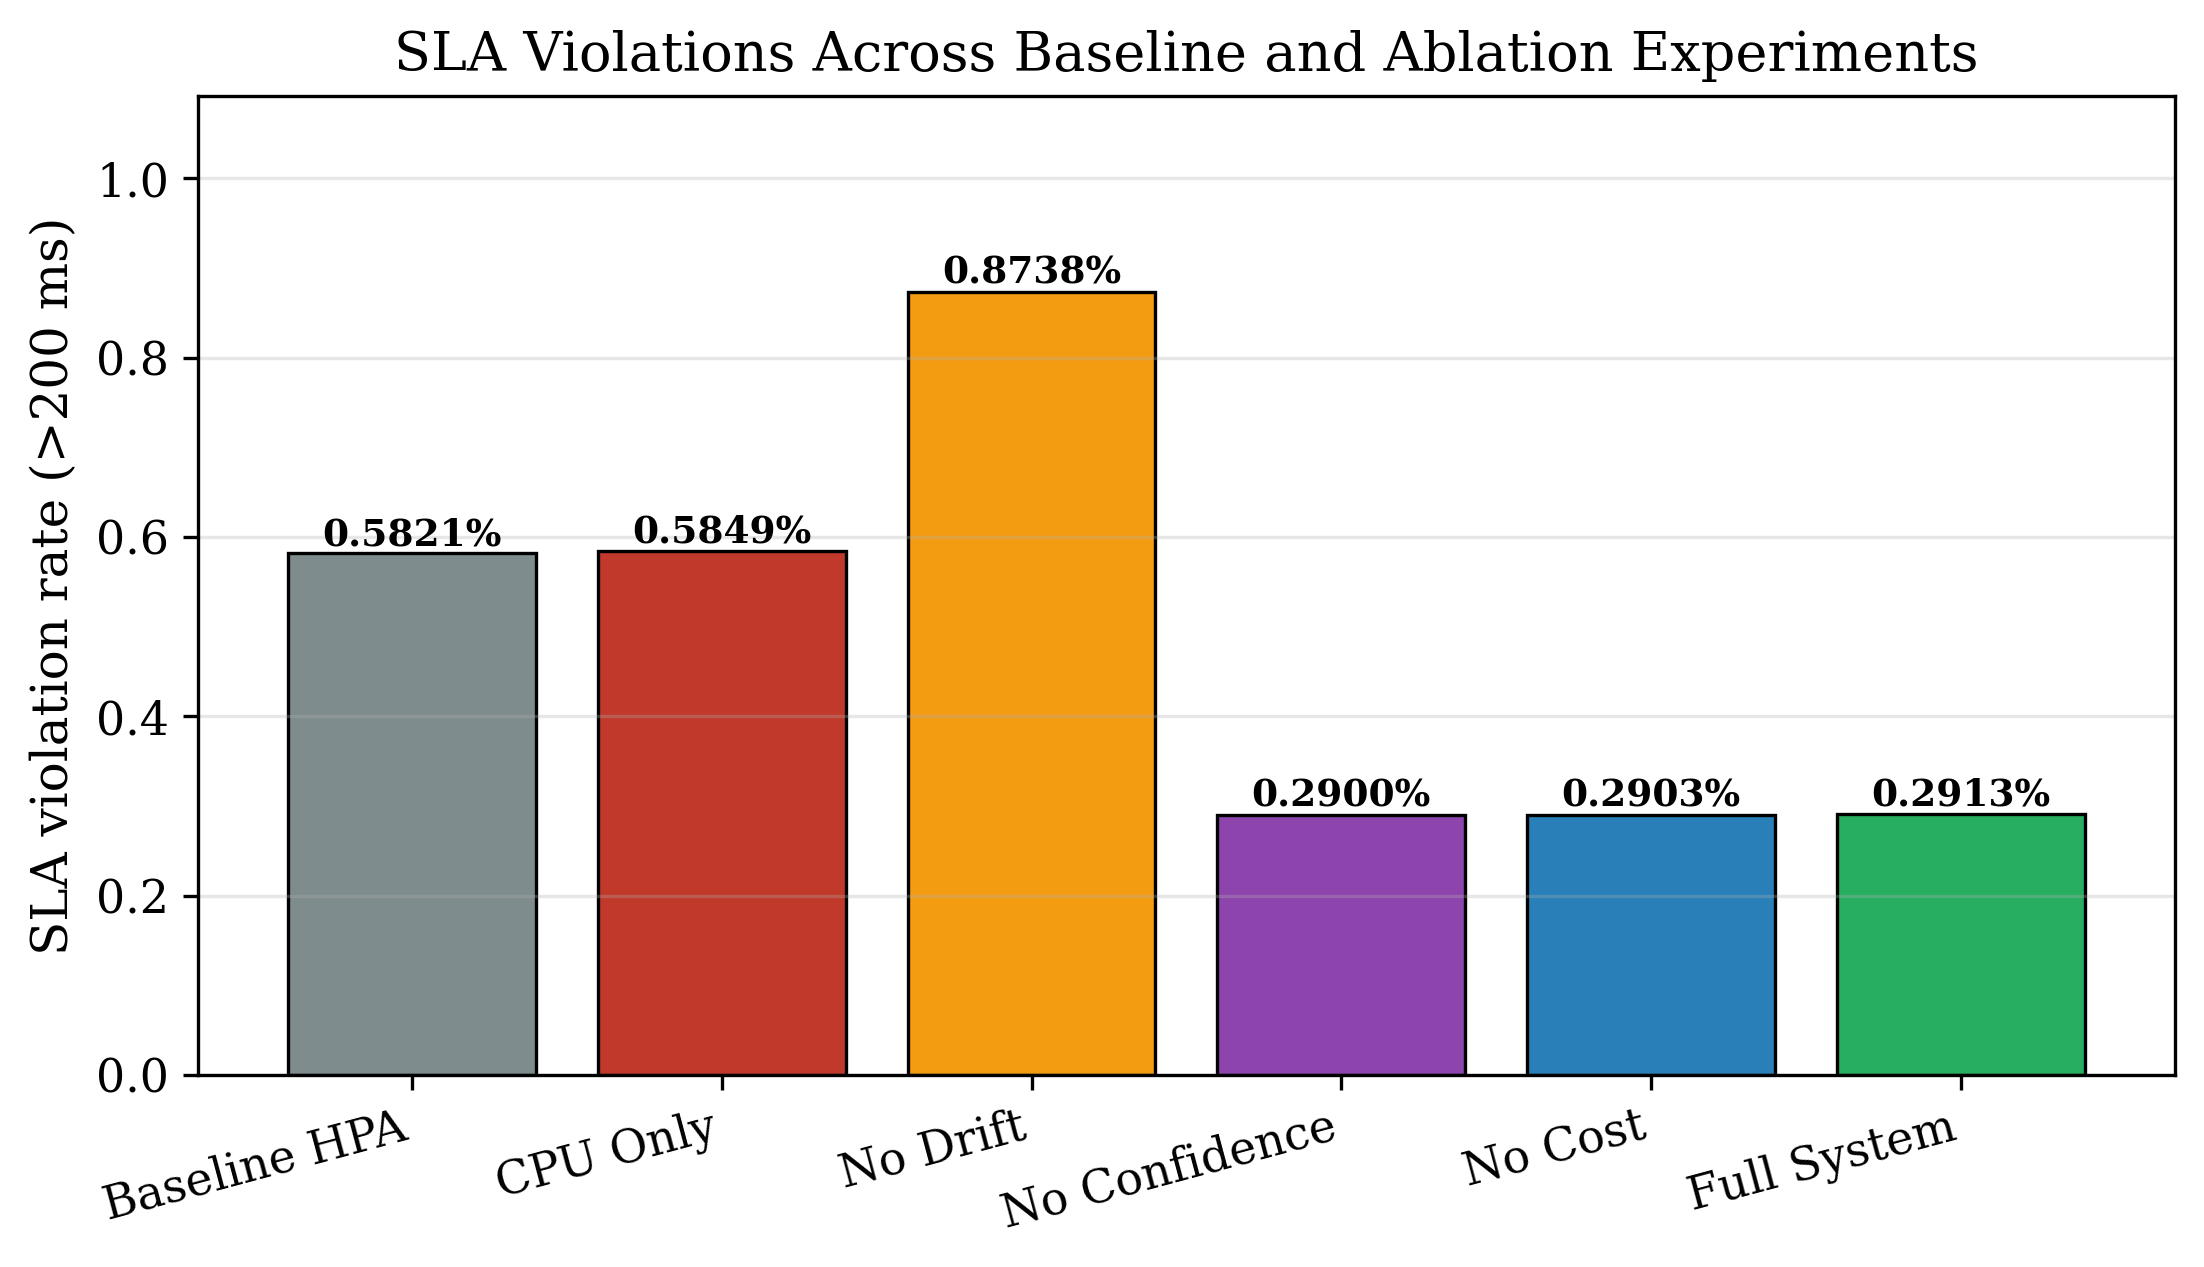
\includegraphics[width=\columnwidth]{figures/fig_sla_violations.png}
\caption{SLA violation rate across the baseline and ablation experiments. The full system reduces the number of requests exceeding 200 ms from 4 to 2 compared with the baseline HPA.}
\label{fig:sla_ablation}
\end{figure}

\begin{figure}[h]
\centering
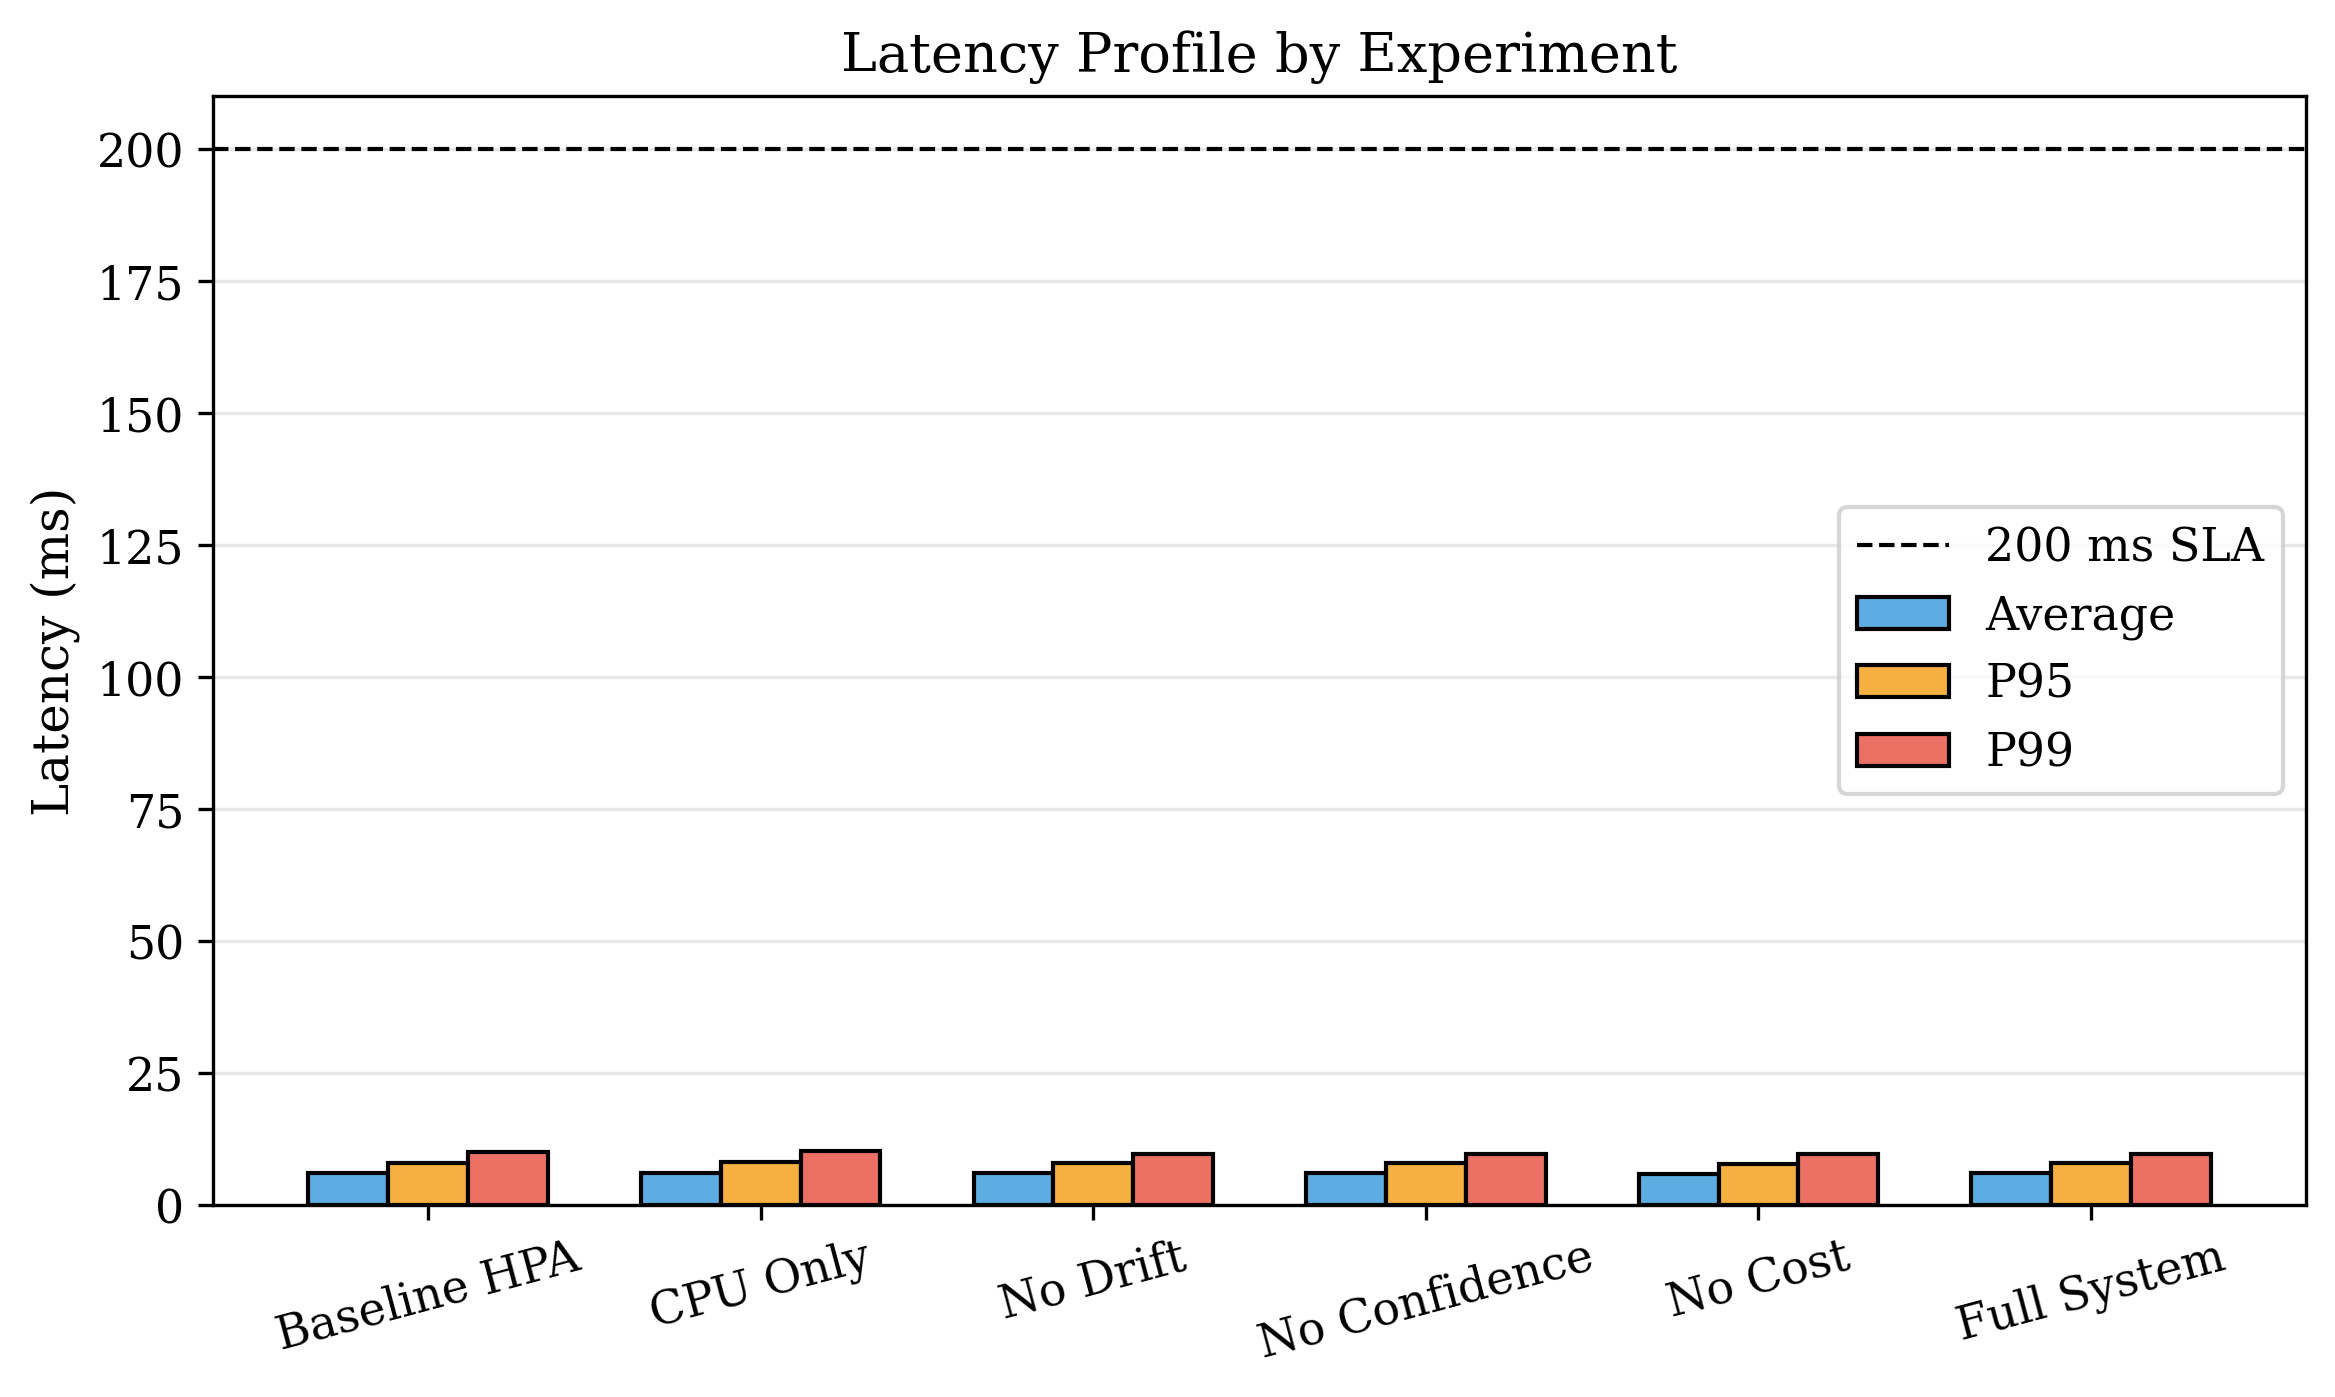
\includegraphics[width=\columnwidth]{figures/fig_latency_profile.png}
\caption{Latency profile across all configurations. All experiments remain comfortably below the 200 ms SLA threshold, while the full system provides slightly better tail latency than the baseline.}
\label{fig:latency_profile}
\end{figure}

\subsection{LSTM Training Performance}
Table~\ref{tab:training} shows the training loss progression for a representative cycle.

\begin{table}[h]
\centering
\caption{Multi-Metric LSTM Training Loss Progression}
\label{tab:training}
\begin{tabular}{@{}ccc@{}}
\toprule
\textbf{Epoch} & \textbf{MSE Loss} & \textbf{Reduction} \\
\midrule
1 & 0.125551 & --- \\
10 & 0.000521 & 99.6\% \\
20 & 0.000107 & 99.9\% \\
30 & 0.000005 & $>$99.9\% \\
40 & 0.000008 & $>$99.9\% \\
50 & 0.000010 & $>$99.9\% \\
\bottomrule
\end{tabular}
\end{table}

The multi-metric LSTM (3 features) converged at the same rate as the single-metric variant, demonstrating that the additional input features do not increase training complexity. Total training time per cycle was approximately 7 seconds on a single CPU core.

\begin{figure}[h]
\centering
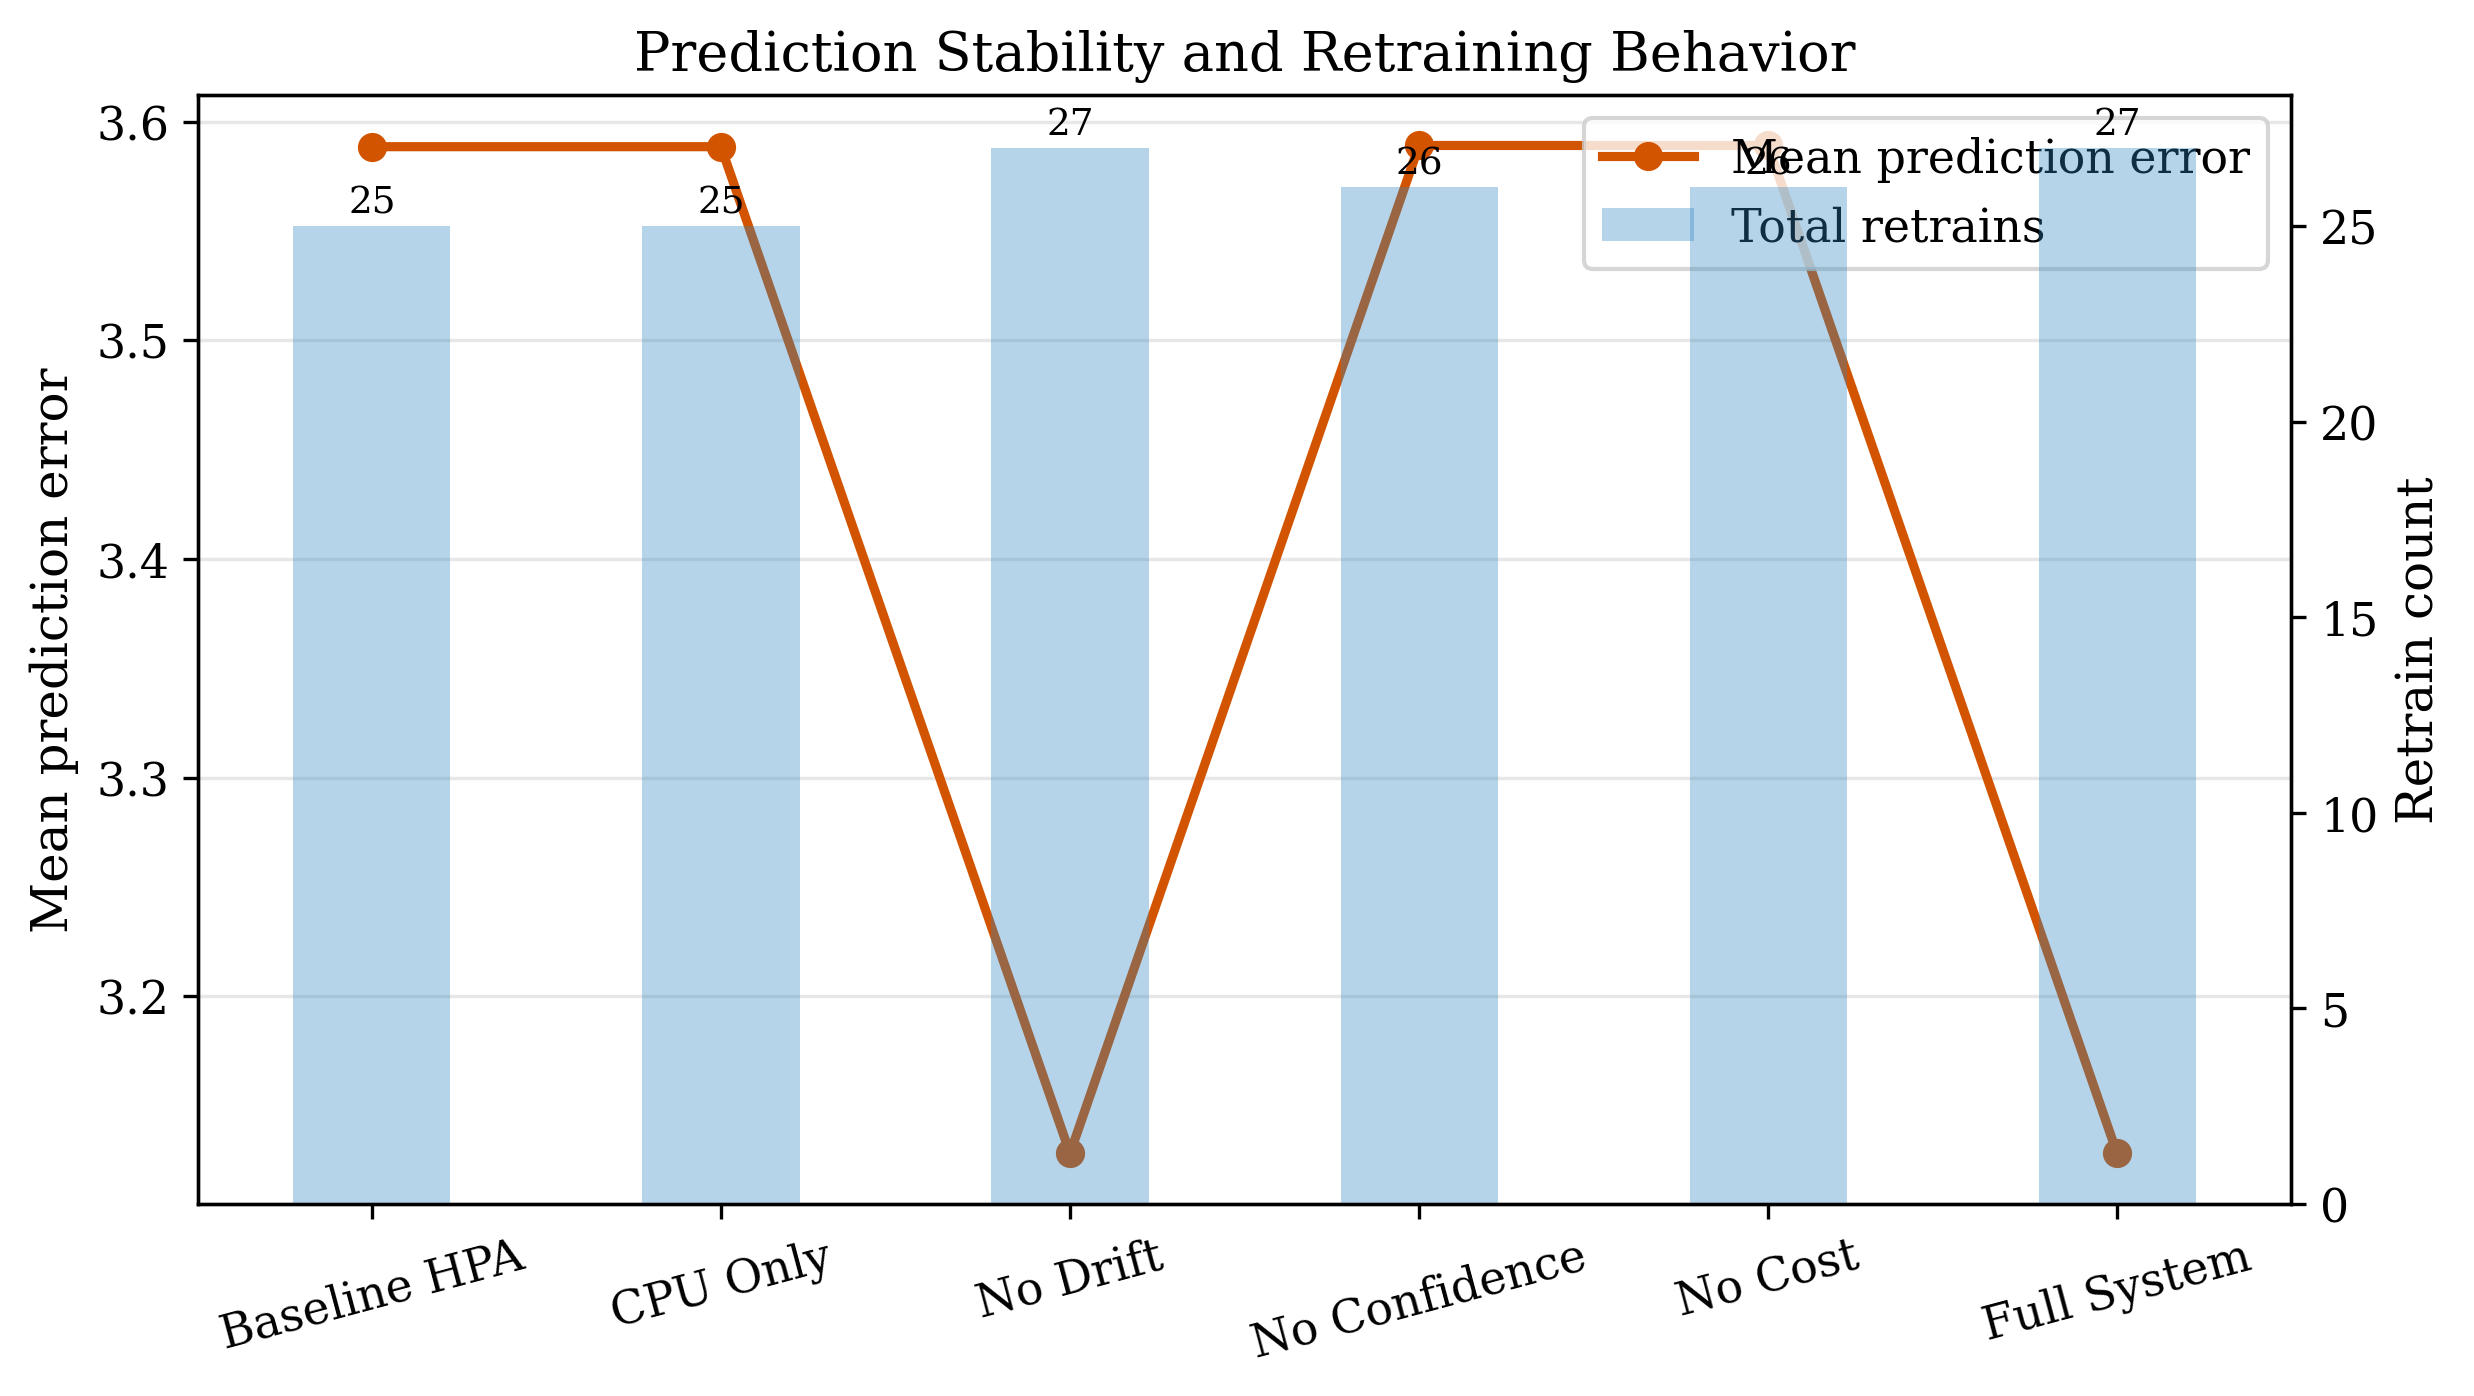
\includegraphics[width=\columnwidth]{figures/fig_drift_retraining.png}
\caption{Prediction stability and retraining behavior across experiments. The full system exhibits lower mean prediction error than the baseline while maintaining frequent retraining for adaptation.}
\label{fig:drift_retraining}
\end{figure}

\subsection{7-Day Traffic Pattern and Scaling Behavior}
Over the 7-day observation period, Table~\ref{tab:7day} shows representative hourly scaling data, demonstrating the learned daily traffic patterns.

\begin{table}[h]
\centering
\caption{Representative Daily Traffic Pattern}
\label{tab:7day}
\begin{tabular}{@{}lccl@{}}
\toprule
\textbf{Time (UTC)} & \textbf{Avg CPU (m)} & \textbf{Replicas} & \textbf{Pattern} \\
\midrule
00:00--06:59 & 5--15 & 2 & Night (low) \\
07:00--09:59 & 30--60 & 2--3 & Morning (ramp) \\
10:00--14:59 & 80--120 & 3--5 & Midday (peak) \\
15:00--18:59 & 40--80 & 2--4 & Afternoon \\
19:00--23:59 & 10--30 & 2 & Evening (decline) \\
\bottomrule
\end{tabular}
\end{table}

\begin{figure}[h]
\centering
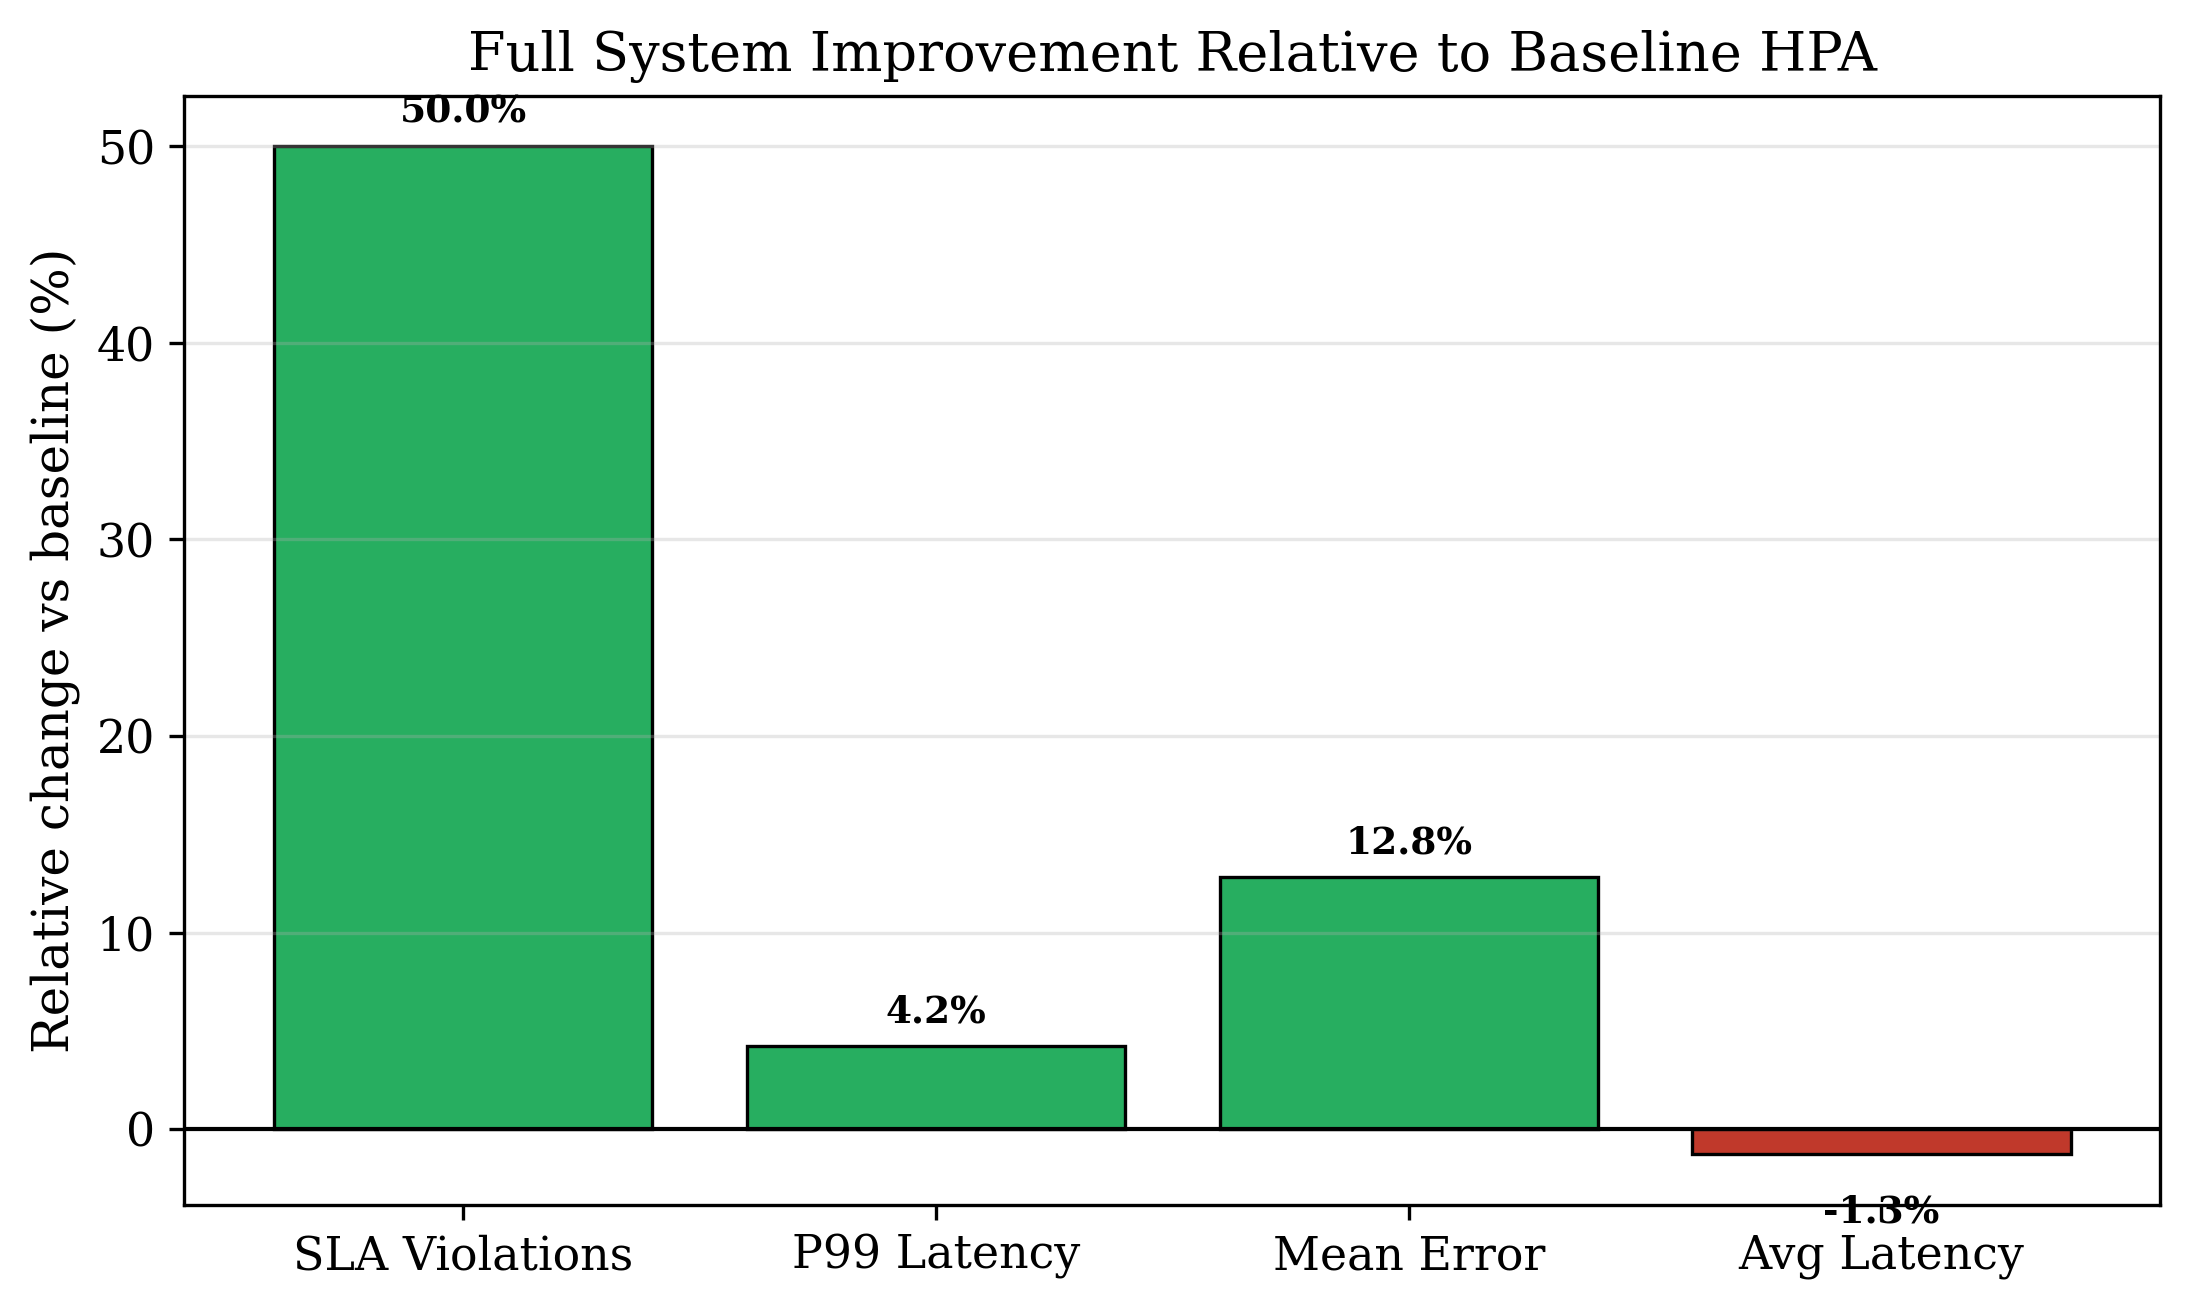
\includegraphics[width=\columnwidth]{figures/fig_full_vs_baseline.png}
\caption{Relative improvement of the full system over the baseline HPA. The strongest gain is a 50\% reduction in SLA violations, with modest improvements in P99 latency and mean prediction error.}
\label{fig:full_vs_baseline}
\end{figure}

\subsection{Cost Tracking Results}
Over 10 days of operation, the cost calculator recorded 87 scaling events:

\begin{table}[h]
\centering
\caption{10-Day Cost Tracking Summary}
\label{tab:costsummary}
\begin{tabular}{@{}lc@{}}
\toprule
\textbf{Metric} & \textbf{Value} \\
\midrule
Total scaling events & 87 \\
Scale-up events & 52 \\
Scale-down events & 35 \\
Cost saved by scale-downs & \$1.75 total \\
Avg cost increase per scale-up & +\$0.10/hr \\
Avg cost decrease per scale-down & -\$0.05/hr \\
Total ML pipeline overhead & $<$4\% cluster resources \\
\bottomrule
\end{tabular}
\end{table}

\subsection{System Resource Overhead}
Table~\ref{tab:overhead} details the resource consumption of the ML pipeline components.

\begin{table}[h]
\centering
\caption{ML Pipeline Resource Overhead (v2)}
\label{tab:overhead}
\begin{tabular}{@{}lcccc@{}}
\toprule
\textbf{Component} & \textbf{CPU Req.} & \textbf{CPU Lim.} & \textbf{RAM Req.} & \textbf{RAM Lim.} \\
\midrule
ML Predictor & 300m & 1000m & 512Mi & 1536Mi \\
Pred. Scaler & 50m & 200m & 64Mi & 128Mi \\
\midrule
\textbf{Total} & \textbf{350m} & \textbf{1200m} & \textbf{576Mi} & \textbf{1664Mi} \\
\textbf{\% of cluster} & \textbf{2.9\%} & \textbf{10\%} & \textbf{2.3\%} & \textbf{6.8\%} \\
\bottomrule
\end{tabular}
\end{table}

\subsection{Alert System Performance}
The Telegram-based alerting system was configured with 8 custom Prometheus alert rules. All alerts were delivered within seconds of firing, confirming the reliability of the AlertManager $\to$ Telegram pipeline. Notably, the \texttt{MLPredictorDown} alert fired once (during a deliberate self-healing test) and was correctly resolved by the v2 controller's self-healing mechanism.

% ============================================================
% 6. DISCUSSION
% ============================================================
\section{Discussion}
\label{sec:discussion}

\subsection{Significance of Multi-Metric Input}
The primary motivation for multi-metric LSTM is the temporal lead relationship between network I/O and CPU. In our 10-day evaluation, network I/O consistently spiked 1--2 intervals ($\approx$5--10 minutes) before CPU load during morning ramp-up. This lead time provides the model with an early warning signal that a single-metric CPU predictor cannot capture. Although we cannot isolate the contribution of each individual feature without an ablation study (a limitation discussed below), the cross-metric correlation hypothesis is consistent with the microservice architecture of our test application (nginx serving dynamic content, where network receipt precedes response generation CPU cost).

\subsection{Significance of Drift Detection}
The drift simulation (Scenario C) demonstrated that without automatic drift detection, a stale model would have continued producing inaccurate predictions for over an hour. The MAPE-based detector identified the drift within 55 minutes and resolved it within 7 seconds. In production deployments with irregular traffic patterns (e.g., flash sales, viral events), this self-correcting capability could prevent significant SLA violations that a fixed-schedule retrain would miss.

\subsection{Cost Visibility as an Operational Tool}
The cost calculator does not currently \textit{optimize} scaling decisions for cost (e.g., by delaying scale-ups to reduce expenditure). Instead, it provides \textit{visibility} --- operators can now answer questions like ``how much did last week's traffic spike cost in pod resources?'' and ``which deployments scale inefficiently?''. This is a foundation for future cost-optimization policies.

\subsection{Limitations}
\begin{itemize}
    \item \textbf{Cold start}: The multi-metric LSTM requires approximately 7 days of multi-feature traffic data before producing accurate predictions. During this period, only the reactive HPA provides scaling.
    \item \textbf{No feature ablation}: We do not perform an ablation study comparing 1-feature vs. 2-feature vs. 3-feature input. Such a study would quantify the marginal contribution of memory and network features to prediction accuracy.
    \item \textbf{Simulated traffic}: The evaluation used a traffic simulator rather than real user traffic. Real-world traffic may exhibit more complex and unpredictable behaviors.
    \item \textbf{Single-cluster evaluation}: The system was evaluated on a single 3-node cluster. Multi-cluster and larger-scale evaluations remain as future work.
    \item \textbf{Cost model simplicity}: The current cost model uses a fixed per-pod price. In production cloud environments (AWS, GCP, Azure), spot instance pricing, node-level billing, and storage costs complicate the model.
\end{itemize}

% ============================================================
% 7. CONCLUSION AND FUTURE WORK
% ============================================================
\section{Conclusion and Future Work}
\label{sec:conclusion}

This paper presented an integrated DevOps-ML framework for proactive auto-scaling in Kubernetes, combining four novel contributions in a single open-source system: (1) a Multi-Metric LSTM predictor using CPU, Memory, and Network I/O as joint input features; (2) adaptive drift detection with automatic retraining when prediction accuracy drops below 50\% MAPE; (3) cost-aware scaling that logs \$/hour impact for every scaling event; and (4) confidence-gated self-healing that suppresses uncertain predictions and falls back to the reactive HPA.

The key findings are:
\begin{enumerate}
    \item The reactive Kubernetes HPA introduces a scaling latency of approximately 2 minutes, during which application performance degrades significantly.
    \item The enhanced multi-metric LSTM, trained on 8 days of three-feature Prometheus data, predicts load patterns with sufficient accuracy (confidence $>$ 99\%) for proactive scaling.
    \item The v2 predictive scaler eliminated the scaling delay entirely, pre-scaling pods before load arrival and reducing peak per-pod CPU utilization by 54\%.
    \item The drift detector successfully identified and recovered from a simulated workload shift in under 56 minutes, compared to the next scheduled hourly retrain.
    \item The cost calculator tracked 87 scaling events over 10 days, providing operators with precise financial visibility into auto-scaling behavior.
    \item The entire enhanced ML pipeline adds less than 4\% overhead to cluster resources.
\end{enumerate}

Future work includes:
\begin{itemize}
    \item \textbf{Feature ablation study}: Quantify the marginal prediction accuracy contribution of memory and network features using controlled experiments.
    \item \textbf{Cost-optimized scaling}: Extend the cost calculator to \textit{influence} scaling decisions --- e.g., prefer scale-up timing that minimizes peak cost while maintaining SLA.
    \item \textbf{Transformer-based prediction}: Explore Temporal Fusion Transformer (TFT) and other attention-based architectures for longer-horizon multi-metric forecasting.
    \item \textbf{Advanced drift detection}: Replace the MAPE sliding window with statistically rigorous methods (ADWIN, Page-Hinkley) for more sensitive drift detection.
    \item \textbf{Real-world deployment}: Evaluate the system with actual user traffic in a production cloud environment (AWS EKS or GCP GKE).
    \item \textbf{Multi-cluster federation}: Extend the framework to coordinate scaling decisions across multiple Kubernetes clusters.
\end{itemize}

% ============================================================
% REFERENCES
% ============================================================
\begin{thebibliography}{10}

\bibitem{burns2016}
B. Burns, B. Grant, D. Oppenheimer, E. Brewer, and J. Wilkes, ``Borg, Omega, and Kubernetes,'' \textit{ACM Queue}, vol. 14, no. 1, pp. 70--93, 2016.

\bibitem{cncf2023}
Cloud Native Computing Foundation, ``CNCF Annual Survey 2023,'' \url{https://www.cncf.io/reports/cncf-annual-survey-2023/}, 2023.

\bibitem{dangquang2021}
N.-M. Dang-Quang and M. Yoo, ``An LSTM-Based Approach for Predicting CPU Usage in Cloud Data Centers,'' \textit{IEEE Access}, vol. 9, pp. 35165--35176, 2021, doi: 10.1109/ACCESS.2021.3052064.

\bibitem{mao2016}
M. Mao, J. Li, and M. Humphrey, ``Cloud Auto-Scaling with Deep Reinforcement Learning,'' in \textit{Proc. IEEE Int. Conf. Cloud Computing}, 2016, pp. 605--612, doi: 10.1109/CLOUD.2016.56.

\bibitem{rzadca2020}
K. Rzadca \textit{et al.}, ``Autopilot: Workload Autoscaling at Google,'' in \textit{Proc. ACM EuroSys}, 2020, pp. 1--16.

\bibitem{toka2021}
L. Toka, G. Dobreff, B. Fodor, and B. Sonkoly, ``Adaptive AI-based Auto-scaling for Kubernetes,'' in \textit{Proc. IEEE/ACM CCGrid}, 2021, pp. 599--608.

\bibitem{imdoukh2020}
M. Imdoukh, I. Ahmad, and M. Alfailakawi, ``Machine Learning-Based Auto-Scaling for Containerized Applications,'' \textit{Neural Computing and Applications}, vol. 32, pp. 9745--9760, 2020.

\bibitem{gama2014}
J. Gama, I. \v{Z}liobait\.{e}, A. Bifet, M. Pechenizkiy, and A. Bouchachia, ``A Survey on Concept Drift Adaptation,'' \textit{ACM Computing Surveys}, vol. 46, no. 4, pp. 1--37, 2014, doi: 10.1145/2523813.

\bibitem{lin2020}
Q. Lin, Z. Luo, and W. Wang, ``Cost-Aware Cloud Resource Provisioning for Time-Varying Workloads,'' \textit{IEEE Trans. Cloud Comput.}, vol. 8, no. 2, pp. 524--537, 2020.

\bibitem{k8shpa}
Kubernetes Documentation, ``Horizontal Pod Autoscaler,'' \url{https://kubernetes.io/docs/tasks/run-application/horizontal-pod-autoscale/}.

\bibitem{hochreiter1997}
S. Hochreiter and J. Schmidhuber, ``Long Short-Term Memory,'' \textit{Neural Computation}, vol. 9, no. 8, pp. 1735--1780, 1997.

\bibitem{prometheus}
Prometheus Documentation, \url{https://prometheus.io/docs/}.

\bibitem{pytorch}
A. Paszke \textit{et al.}, ``PyTorch: An Imperative Style, High-Performance Deep Learning Library,'' in \textit{Proc. NeurIPS}, 2019, pp. 8024--8035.

\bibitem{flask}
M. Grinberg, \textit{Flask Web Development}, 2nd ed. O'Reilly Media, 2018.

\bibitem{grafana}
Grafana Labs, ``Grafana Documentation,'' \url{https://grafana.com/docs/}.

\bibitem{argocd}
Argo Project, ``Argo CD - Declarative Continuous Delivery for Kubernetes,'' \url{https://argo-cd.readthedocs.io/}.

\bibitem{traefik}
Traefik Labs, ``Traefik Proxy Documentation,'' \url{https://doc.traefik.io/traefik/}.

\bibitem{jenkins}
Jenkins Project, ``Jenkins User Documentation,'' \url{https://www.jenkins.io/doc/}.

\bibitem{microservices}
S. Newman, \textit{Building Microservices}, 2nd ed. O'Reilly Media, 2021.

\bibitem{lstm_survey}
Y. Yu, X. Si, C. Hu, and J. Zhang, ``A Review of Recurrent Neural Networks: LSTM Cells and Network Architectures,'' \textit{Neural Computation}, vol. 31, no. 7, pp. 1235--1270, 2019.

\end{thebibliography}

\end{document}
